%%%%%%%%%%%%%%%%%%%%%%%%%%%%%%%%%
% Background and Literature Review
%%%%%%%%%%%%%%%%%%%%%%%%%%%%%%%%%

\section{BACKGROUND AND LITERATURE REVIEW}

This section establishes the theoretical and empirical foundations of this work. The background subsection introduces the key concepts in sound synthesis, the formal definition of the inverse synthesis problem, and the audio representations used as model inputs. The literature review then surveys prior work, moving from early optimization-based methods to modern deep learning approaches, and identifies the gap this study addresses.

\subsection{Background}

\subsubsection{Sound Synthesis and the Vital Synthesizer}

\subsubsubsection{A Brief History of Sound Synthesis}

The development of electronic sound synthesis spans six decades and four distinct technological paradigms, each shifting both the physics of sound generation and the sonic vocabulary of popular music \cite{roads1996computer}.

\par \vspace{0.3cm}

\noindent \textbf{Analog synthesis (1960s--1980s).} Robert Moog's demonstration of the first voltage-controlled synthesizer at the 1964 Audio Engineering Society convention established the foundational architecture that underlies all modern synthesizers: a voltage-controlled oscillator (VCO) generating a periodic waveform, a voltage-controlled filter (VCF) shaping its spectral content, and a voltage-controlled amplifier (VCA) imposing its dynamic envelope. The Minimoog Model D (1970) condensed this modular system into a portable, self-contained instrument whose normalled signal chain --- oscillators into filter into amplifier into effects --- remains the canonical template to this day. The ARP 2600 (1971) offered a semi-modular alternative prized for its patchable flexibility. The Prophet-5 (Sequential Circuits, 1978) introduced full programmability and patch memory to a polyphonic synthesizer, allowing sounds to be saved and recalled exactly --- a capability so fundamental that it is taken for granted in every instrument that followed \cite{cook2002realsound}.

\par \vspace{0.3cm}

\noindent These instruments defined the sonic palette of rock, funk, and early electronic music. Keith Emerson's Moog solo on ``Lucky Man'' by Emerson, Lake \& Palmer (1970) was one of the first widely heard synthesizer performances on a rock record. Stevie Wonder's \textit{Talking Book} (1972) and \textit{Innervisions} (1973) used the Minimoog as a primary melodic voice. Kraftwerk's ``Autobahn'' (1974) and Giorgio Moroder's sequenced Moog bassline on Donna Summer's ``I Feel Love'' (1977) established the synthesizer as a self-sufficient compositional medium. The ARP 2600 reached a different kind of cultural permanence: sound designer Ben Burtt used it to construct the voice of R2-D2 in \textit{Star Wars} (1977). The Prophet-5 contributed the thick polyphonic pads and brass stabs of synth-pop, heard across the work of Tears for Fears, Peter Gabriel, and New Order throughout the 1980s.

\par \vspace{0.3cm}

\noindent \textbf{Rhythm synthesis: the TR-808 and TB-303 (1980--1981).} Though not melodic synthesizers in the traditional sense, the Roland TR-808 drum machine and TB-303 bass line synthesizer represent milestone achievements in analog circuit-based sound generation. The TR-808 synthesized kick drums, snares, and hi-hats entirely from analog circuits rather than recorded samples, producing a distinctive deep kick and crisp rimshot that became the rhythmic foundation of hip-hop and electronic music. Afrika Bambaataa's ``Planet Rock'' (1982), Marvin Gaye's ``Sexual Healing'' (1982), and Prince's ``When Doves Cry'' (1984) brought the 808 to mainstream attention; it subsequently became the defining rhythmic voice of trap music. The TB-303 bass synthesizer, equipped with a resonant filter that could be driven to extreme squelching self-oscillation, gave an entire genre its name: Phuture's ``Acid Tracks'' (1987) launched acid house and, by extension, the lineage of techno and electronic dance music.

\par \vspace{0.3cm}

\noindent \textbf{FM and digital synthesis (1980s).} The Yamaha DX7 (1983) replaced analog circuits with six-operator frequency modulation (FM) synthesis, in which a set of digital oscillators modulate each other's frequencies to produce complex sideband-rich spectra unavailable to analog filters. The DX7 sold over 200,000 units, making it the best-selling synthesizer in history \cite{roads1996computer}, and its factory presets --- particularly the electric piano, slap bass, and marimba patches --- appeared on virtually every commercially released pop record between 1983 and 1990. A-ha's ``Take On Me'' (1985) and the prolific output of Quincy Jones's productions in this era are among the most recognizable examples. The Roland D-50 (1987) introduced linear arithmetic synthesis, blending short PCM attack transients with digital sustain bodies to produce lush, layered sounds that defined late-1980s new age and film scoring.

\par \vspace{0.3cm}

\noindent \textbf{Sample-based synthesis (late 1980s--2000s).} The Fairlight CMI (1979) and New England Digital Synclavier were the first instruments to store and play back arbitrary recorded waveforms at different pitches --- a paradigm shift from generating sound to reproducing it. Both were prohibitively expensive; Kate Bush used the Fairlight on ``Running Up That Hill'' (1985), and the Synclavier is audible across Michael Jackson's \textit{Thriller} (1982) productions. The Akai S950 and S1000 brought professional-quality sampling to a broader market and became central to 1990s hip-hop production. The Korg M1 (1988) combined sample playback with onboard effects and became the best-selling keyboard workstation of all time; its organ and piano presets are inseparable from the sound of early house music, heard on Black Box's ``Ride on Time'' (1989). This era shifted the craft of sound design from building timbres from physical first principles to selecting, layering, and processing recorded material.

\par \vspace{0.3cm}

\noindent \textbf{Software synthesis (1996--present).} Steinberg's VST (Virtual Studio Technology) standard in 1996 opened the digital audio workstation to third-party software instruments, eliminating the need for dedicated hardware. Software synthesizers could now implement any synthesis paradigm at negligible cost and with perfect parameter recall. Native Instruments, Arturia, and others recreated classic hardware digitally, free from tuning drift and with unlimited voices. Vital (Matt Tytel, 2020) represents the current endpoint of this trajectory: a free, open-source wavetable synthesizer that combines the classic analog signal chain with arbitrary wavetable oscillators, a deep modulation matrix, and programmatic parameter access via API. This evolution --- from a room-sized modular Moog to a synthesizer anyone can run on a laptop and control from a Python script --- is precisely what makes the inverse synthesis problem both tractable to study and practically relevant for working musicians.

\par \vspace{0.3cm}

\noindent Table~\ref{tab:synthesis_paradigms} summarises the four main synthesis paradigms discussed above.

\begin{table}[H]
\centering
\renewcommand{\arraystretch}{1.4}
\begin{tabular}{p{2.6cm} p{2.8cm} p{4.2cm} p{4.0cm}}
\hline
\textbf{Era} & \textbf{Paradigm} & \textbf{Key Instruments} & \textbf{Core Mechanism} \\
\hline
1960s--1980s & Analog subtractive & Moog Modular, Minimoog, ARP 2600, Prophet-5 & VCO waveforms shaped by VCF and VCA via continuous voltage control \\
1980s & FM / digital & Yamaha DX7, Roland D-50 & Digital oscillators modulating each other's frequencies to produce sideband-rich spectra \\
Late 1980s--2000s & Sample-based & Fairlight CMI, Akai S-Series, Korg M1 & PCM recordings played back at different pitches and shaped by digital filters \\
1996--present & Software (VST) & Native Instruments, Arturia, Vital & Any synthesis algorithm running inside a DAW with no dedicated hardware \\
\hline
\end{tabular}
\vspace{0.3cm}
\caption{The four main sound synthesis paradigms from the analog era to modern software synthesizers.}
\label{tab:synthesis_paradigms}
\end{table}

\subsubsubsection{Physics of Electronic Sound Generation}

Understanding the physical mechanisms behind synthesis is essential for interpreting which properties of an audio representation carry the most information for parameter estimation.

\par \vspace{0.3cm}

\noindent \textbf{Oscillators.} An oscillator generates a periodic waveform defined by three properties: frequency (perceived as pitch), amplitude (perceived as loudness), and waveform shape (perceived as timbre). The most common synthesizer waveforms differ in their harmonic content, which can be expressed analytically via the Fourier series. A sawtooth wave at fundamental frequency $f_0$ contains energy at all integer harmonics ($f_0, 2f_0, 3f_0, \ldots$) with amplitudes decreasing as $1/n$, producing a spectrally rich, bright timbre ideal for subtractive shaping. A square wave contains only odd harmonics ($f_0, 3f_0, 5f_0, \ldots$), giving it a hollow, nasal quality. A sine wave carries energy only at $f_0$ with no harmonics. In analog circuits, sawtooth waves are generated by the linear charge of a capacitor followed by a rapid discharge; in digital synthesis, these waveforms are stored as lookup tables read at a rate proportional to the desired pitch. Table~\ref{tab:waveforms} summarises the harmonic structure of the four fundamental waveforms.

\begin{table}[H]
\centering
\renewcommand{\arraystretch}{1.4}
\begin{tabular}{p{2.3cm} p{4.5cm} p{2.8cm} p{4.0cm}}
\hline
\textbf{Waveform} & \textbf{Harmonics present} & \textbf{Amplitude roll-off} & \textbf{Spectral character} \\
\hline
Sine     & Fundamental $f_0$ only                              & ---         & Pure tone; no overtones \\
Sawtooth & All harmonics ($f_0, 2f_0, 3f_0, \ldots$)          & $1/n$       & Bright, spectrally rich; standard subtractive source \\
Square   & Odd harmonics only ($f_0, 3f_0, 5f_0, \ldots$)     & $1/n$       & Hollow, nasal; roughly half the energy of sawtooth \\
Triangle & Odd harmonics only ($f_0, 3f_0, 5f_0, \ldots$)     & $1/n^2$     & Soft, mellow; harmonics decay far faster than square \\
\hline
\end{tabular}
\vspace{0.3cm}
\caption{Harmonic content of the four fundamental synthesizer oscillator waveforms, derived from their Fourier series representations.}
\label{tab:waveforms}
\end{table}

\par \vspace{0.3cm}

\noindent \textbf{Filters (VCF).} A voltage-controlled filter shapes the spectral content of the oscillator output by attenuating energy above or below a cutoff frequency. In a low-pass filter --- the most common type in subtractive synthesis --- frequencies above the cutoff are attenuated at a slope determined by the filter order (typically 2-pole or 4-pole, corresponding to $-12$ or $-24$ dB per octave). The resonance parameter (also called $Q$) introduces a narrow peak in the filter's frequency response at the cutoff frequency; at high resonance settings, this peak amplifies a narrow spectral band dramatically. At extreme resonance values the filter enters self-oscillation, generating a near-pure sine tone independently of the oscillator input. The Moog transistor ladder filter --- a 4-pole design --- introduced a characteristic phase shift and warmth that became the defining timbral component of the analog era. The filter cutoff is expressed in semitones in Vital, rather than in Hz, reflecting the exponential relationship between MIDI pitch and frequency ($f = 440 \cdot 2^{(p-69)/12}$) and directly motivating the logarithmic normalization applied to this parameter during training.

\par \vspace{0.3cm}

\noindent \textbf{Envelopes (ADSR).} An envelope generator produces a time-varying control signal that modulates either the VCA (amplitude envelope, Envelope 1 in this work) or the VCF cutoff (filter envelope, Envelope 2). The standard ADSR shape is defined by four stages: \textit{Attack} (time to rise from zero to peak after a note-on event), \textit{Decay} (time to fall from peak to the sustain level), \textit{Sustain} (the held level while the key remains pressed), and \textit{Release} (time to fall to zero after note-off). In Vital, attack and decay times are internally quantized to 1001 logarithmically spaced values spanning several orders of magnitude, reflecting the perceptual importance of fine distinctions at short durations and coarser ones at long durations. This directly motivates the $\log_{10}$ normalization applied to all envelope time parameters before training. The sustain and release stages are excluded from this study: the fixed 4-second render without a note-off event makes both stages unobservable from the audio. Figure~\ref{fig:adsr} illustrates the full ADSR shape and highlights the two stages used in this work.

\begin{figure}[H]
\centering
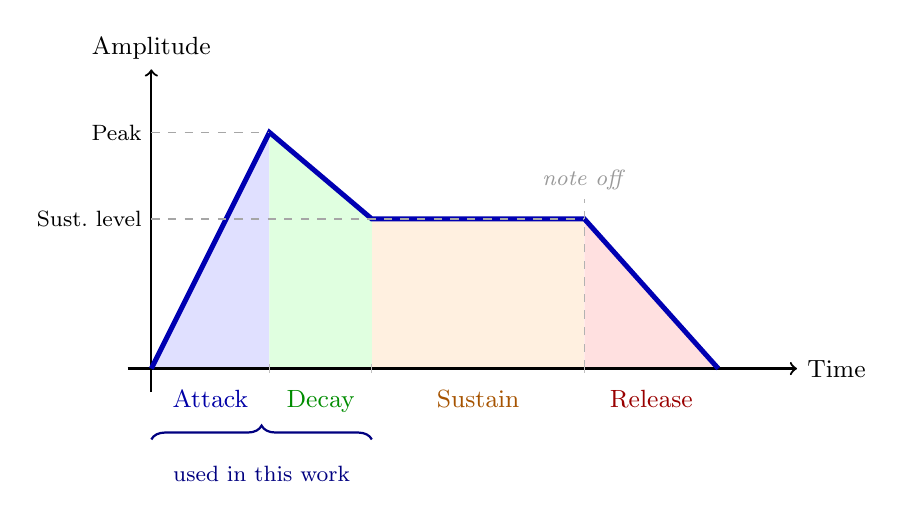
\begin{tikzpicture}
  % Stage shading (drawn first, under envelope line)
  \fill[blue!12]   (0,0) -- (1.5,3.0) -- (1.5,0) -- cycle;
  \fill[green!12]  (1.5,0) -- (1.5,3.0) -- (2.8,1.9) -- (2.8,0) -- cycle;
  \fill[orange!12] (2.8,0) rectangle (5.5,1.9);
  \fill[red!12]    (5.5,0) -- (5.5,1.9) -- (7.2,0) -- cycle;

  % Axes
  \draw[thick, ->] (-0.3,0) -- (8.2,0) node[right, font=\small] {Time};
  \draw[thick, ->] (0,-0.3) -- (0,3.8) node[above, font=\small] {Amplitude};

  % ADSR envelope line
  \draw[blue!70!black, line width=1.8pt]
    (0,0) -- (1.5,3.0) -- (2.8,1.9) -- (5.5,1.9) -- (7.2,0);

  % Dashed reference lines
  \draw[dashed, gray!70] (0,3.0) -- (1.5,3.0);
  \draw[dashed, gray!70] (0,1.9) -- (5.5,1.9);
  \node[left, font=\footnotesize] at (0,3.0) {Peak};
  \node[left, font=\footnotesize] at (0,1.9) {Sust.\ level};

  % Note-off dashed vertical line
  \draw[dashed, gray!60] (5.5,0) -- (5.5,2.15);
  \node[above, font=\footnotesize, gray!80] at (5.5,2.15) {\textit{note off}};

  % Stage boundary ticks on x-axis
  \foreach \x in {1.5, 2.8, 5.5} {
    \draw[gray!50] (\x,0.06) -- (\x,-0.06);
  }

  % Stage labels below x-axis
  \node[below=0.15cm, font=\small, blue!65!black]   at (0.75,0) {Attack};
  \node[below=0.15cm, font=\small, green!55!black]  at (2.15,0) {Decay};
  \node[below=0.15cm, font=\small, orange!65!black] at (4.15,0) {Sustain};
  \node[below=0.15cm, font=\small, red!60!black]    at (6.35,0) {Release};

  % Annotation for stages used in this work
  \draw[decorate, decoration={brace, amplitude=5pt}, thick, blue!50!black]
    (0, -0.9) -- (2.8, -0.9)
    node[midway, below=6pt, font=\footnotesize, blue!50!black] {used in this work};
\end{tikzpicture}
\vspace{0.3cm}
\caption{The ADSR (Attack, Decay, Sustain, Release) envelope shape. A note-on event triggers the Attack; the Decay brings the level down to Sustain, which is held while the key is pressed; Release begins at note-off. Only the Attack and Decay stages are studied here, as all audio clips are fixed 4-second renders with no note-off event. Envelope~1 drives the VCA (amplitude); Envelope~2 drives the filter cutoff, with \texttt{modulation\_1\_amount} controlling the modulation depth.}
\label{fig:adsr}
\end{figure}

\par \vspace{0.3cm}

\noindent \textbf{Voltage-controlled amplifier (VCA).} The VCA multiplies the filtered oscillator signal by the amplitude envelope, imposing the dynamic contour of the sound. Together, the oscillator, filter, and VCA constitute the complete subtractive synthesis signal chain: \textit{Oscillator(s) $\rightarrow$ Filter $\rightarrow$ VCA $\rightarrow$ Effects}. This chain, illustrated in Figure~\ref{fig:synthesis_drivers}, corresponds directly to the four parameter groups studied in this work.

\begin{figure}[H]
\centering
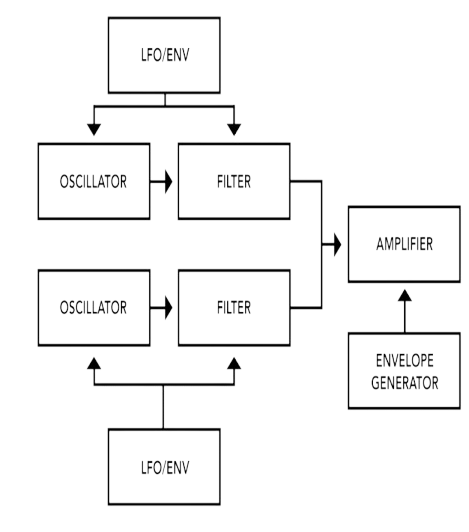
\includegraphics[width=12cm]{images/synthesis_signal_flow.png}
\vspace{0.3cm}
\caption{Signal flow of a subtractive synthesizer, illustrating the key components --- oscillators, filter, envelopes, and effects --- that correspond to the 16 parameters studied in this work \cite{cymatics_subtractive}.}
\label{fig:synthesis_drivers}
\end{figure}

\subsubsubsection{Wavetable Synthesis and the Vital Synthesizer}

\textit{Wavetable synthesis} was introduced by Wolfgang Palm in the PPG Wave synthesizer (1981) and extends the classic oscillator paradigm by replacing a fixed waveform shape with a table of up to 256 single-cycle waveforms. Rather than generating a mathematically defined waveform, the oscillator reads a slice of this table --- the \textit{wave frame} --- and plays it back at the desired pitch. As the wave frame position parameter is swept continuously, the oscillator morphs between successive frames, producing timbral evolution that is not achievable with fixed waveform shapes.

\par \vspace{0.3cm}

\noindent This paradigm has a fundamental implication for inverse synthesis. In FM synthesis, the output spectrum is analytically computable from the operator ratios and modulation indices: a closed-form relationship exists between parameters and spectral content. In subtractive synthesis, the harmonic series of a sawtooth wave is fixed and predictable; the filter shapes it in a mathematically characterizable way. In wavetable synthesis, the spectral content at any wave frame position is determined entirely by the arbitrary waveform data stored in the table. No closed-form relationship exists between the wave frame parameter and the resulting spectrum, and the interaction between wavetable position, unison voice count, inter-voice detune, and the downstream filter produces a high-dimensional, non-linear mapping from parameters to audio that is substantially harder to invert. This opacity is one of the key motivations for the data-driven regression approach taken in this work, and distinguishes Vital from the FM and subtractive synthesizers studied in most prior inverse synthesis research.

\par \vspace{0.3cm}

\noindent Vital is a modern open-source wavetable synthesizer developed by Matt Tytel and released in 2020. It provides two independent wavetable oscillators, each with its own wave frame position, output level, unison voice count, and inter-voice detune. These feed into the classic subtractive signal chain: a resonant filter, amplitude and filter envelope generators, and an effects section including reverb. Unison stacks multiple detuned copies of an oscillator, producing the characteristic width and thickness of contemporary electronic music sounds. The parameter space studied in this work is restricted to 16 controls --- drawn from the oscillators, filter, envelopes, and effects --- inspired by the fixed signal flow of vintage analog synthesizers. Even with modern synthesizers that expose hundreds of parameters, professional producers consistently rely on a small, interpretable subset \cite{cook2002realsound}; restricting the parameter space keeps the regression task tractable while retaining expressive coverage. Vital's open-source nature and programmatic parameter access via the Pedalboard Python library make it uniquely suited for large-scale, reproducible dataset generation, which is central to the methodology described in Section~\ref{sec:methodology}.

\subsubsection{The Inverse Synthesis Problem}

The inverse synthesis problem is formally defined as follows. Let $\mathbf{y}$ denote an audio signal rendered by a synthesizer $\mathcal{S}$ with parameter vector $\mathbf{x} \in [0,1]^N$, such that $\mathbf{y} = \mathcal{S}(\mathbf{x}, p)$, where $p$ is the MIDI pitch at which the note is played. Given $\mathbf{y}$ and $p$, the goal is to recover an estimate $\hat{\mathbf{x}}$ that is as close as possible to the ground-truth $\mathbf{x}$. In this work, $N = 16$.

\par \vspace{0.5cm}

\noindent The problem is inherently challenging for several reasons. First, the mapping from parameters to audio is \textit{highly non-linear}: small changes in certain parameters (e.g., filter resonance near self-oscillation, unison detune at high voice counts) can produce disproportionately large perceptual changes, while large changes in others (e.g., reverb mix at low values) may be nearly imperceptible. Second, the problem is \textit{ill-posed}: multiple distinct parameter configurations can produce perceptually similar or identical sounds. This many-to-one relationship makes the inverse mapping ambiguous and complicates loss function design. Third, parameters are \textit{interdependent}: the perceptual effect of the filter cutoff, for example, depends on the current envelope modulation depth and the oscillator content feeding into it.

\subsubsection{Audio Representations}

The choice of input representation is critical for audio-based regression tasks. Raw waveforms carry full information but are high-dimensional and difficult to process directly with standard architectures. The Short-Time Fourier Transform (STFT) decomposes a signal into a two-dimensional time-frequency representation by applying a windowed DFT at successive frames. The magnitude of the STFT, known as the spectrogram, discards phase information but retains the spectral energy distribution over time, which is sufficient for characterizing synthesis parameters.

\par \vspace{0.5cm}

\noindent The \textit{mel spectrogram} applies a perceptually motivated frequency scale — the mel scale — which compresses high frequencies and expands low frequencies to approximate the resolution of the human auditory system. This representation has become the standard input for audio classification and regression tasks \cite{hershey2017cnn}. A key design trade-off in mel spectrogram computation is the choice of FFT window size and hop length: short windows provide high temporal resolution at the cost of frequency resolution, while long windows provide high frequency resolution at the cost of temporal smearing. For a task spanning parameters as diverse as attack transients (millisecond-scale) and harmonic structure (tens of milliseconds), no single scale is optimal for all parameters. This motivates the multi-scale representation introduced in V2 of this work, where three spectrograms computed at fine, mid, and coarse resolutions are combined into a three-channel input tensor.

\subsection{Literature Review}

\subsubsection{Optimization-Based Inverse Synthesis}

The earliest systematic approaches to synthesizer parameter estimation relied on iterative search. \textit{Genetic Algorithms} (GAs) encode candidate parameter vectors as individuals in a population and evolve them over successive generations using crossover and mutation operators, guided by an audio similarity fitness function \cite{walker2007audiosynthesis}. While GAs are capable of exploring non-convex parameter spaces without gradient information, they require thousands of synthesizer renders per run and do not generalize: a new search must be run from scratch for each target sound. \textit{Hill-climbing} methods — gradient-free local search — share the same limitations and are additionally prone to getting trapped in local optima in high-dimensional, non-convex spaces. These methods have been applied successfully to simple FM and subtractive synthesizers with few parameters, but scale poorly to complex VSTs like Vital.

\subsubsection{Deep Learning for Direct Parameter Regression}

The shift to deep learning reformulated inverse synthesis as a supervised regression problem: a neural network is trained on a large dataset of audio/parameter pairs and learns to predict parameters directly from an audio representation, eliminating the need for iterative synthesis at inference time.

\par \vspace{0.5cm}

\noindent Yee-King et al. \cite{yeeking2018automatic} were among the first to apply deep networks to VST synthesizer programming, demonstrating that multilayer perceptrons trained on spectral features could outperform genetic algorithms on a commercial soft-synth. Barkan et al. \cite{barkan2019inversynth} introduced \textit{InverSynth}, which applied CNNs to the parameter estimation of an FM synthesizer, framing the task as a multi-output regression problem and establishing the use of mel-spectrograms as the primary input representation. InverSynth II \cite{barkan2023inversynth2} extended this work with self-supervised pre-training and inference-time fine-tuning, improving generalization to unseen sounds. Chen et al. \cite{chen2022sound2synth} proposed \textit{Sound2Synth} for FM synthesis parameter estimation using a transformer encoder, demonstrating the applicability of attention-based models to this task.

\par \vspace{0.5cm}

\noindent A common limitation of these works is their focus on FM synthesizers, which have a well-defined and mathematically tractable parameter-to-sound relationship. Wavetable synthesizers like Vital, where the oscillator timbre is determined by an arbitrary wave frame position and the interaction with a filter and modulation chain, present a more complex and less structured mapping that has received comparatively little attention.

\subsubsection{Differentiable Synthesis}

A parallel line of research has explored making the synthesis process itself differentiable, enabling gradient-based optimization of parameters directly in the audio domain. Engel et al. \cite{engel2020ddsp} introduced \textit{DDSP} (Differentiable Digital Signal Processing), a framework that reimplements synthesis operators — harmonic oscillators, filtered noise, reverb — as differentiable modules in a neural network computation graph. This allows training with perceptual audio losses such as the Multi-Scale Spectral (MSS) loss, which measures reconstruction quality at multiple time-frequency resolutions, and has produced compelling results for instrumental sound synthesis and timbre transfer.

\par \vspace{0.5cm}

\noindent Caspe et al. \cite{caspe2022ddx7} extended this paradigm to FM synthesis with \textit{DDX7}, a differentiable implementation of the Yamaha DX7 architecture that enables end-to-end gradient-based sound matching using spectral losses. Uzrad et al. \cite{diffmoog} introduced \textit{DiffMoog}, a differentiable modular synthesizer designed specifically for sound matching, which enables gradient-based optimization of parameters through a differentiable implementation of a Moog-style synthesis chain.

\par \vspace{0.5cm}

\noindent While these approaches are powerful, they share a fundamental requirement: the synthesizer must be re-implemented as a differentiable module. This is feasible for mathematically well-defined synthesizers (FM, additive, physical models) but is not practical for a production VST like Vital, which operates as a non-differentiable black-box plugin. Constructing a differentiable proxy of Vital would require significant additional engineering effort beyond the scope of this work. For this reason, the MSS loss is used in this study as a \textit{post-hoc evaluation metric} only — not as a training objective — and the supervised regression approach over fixed input-output pairs remains the appropriate framework.

\subsubsection{Deep Learning Architectures for Audio}

\subsubsubsection{Convolutional Neural Networks}
CNNs were among the first deep architectures applied to large-scale audio classification, with Hershey et al. \cite{hershey2017cnn} demonstrating strong performance on AudioSet using standard image classification networks applied to log-mel spectrograms. The key insight — that a mel spectrogram can be treated as a 2D image and processed with convolutional feature extractors — established the template for audio deep learning. He et al. \cite{he2016resnet} introduced residual connections (\textit{ResNets}), which enable training of very deep networks by providing gradient shortcuts and form the backbone of the custom CNN baseline used in this work.

\subsubsubsection{Vision Transformers and AST}
Dosovitskiy et al. \cite{dosovitskiy2021vit} introduced the Vision Transformer (ViT), which patches an image into non-overlapping tokens and processes them with a standard Transformer encoder \cite{vaswani2017attention}. Global self-attention allows ViT to capture long-range spatial dependencies that are difficult for local convolutions to model. Gong et al. \cite{gong2021ast} adapted ViT to audio by pre-training on AudioSet spectrograms, yielding the \textit{Audio Spectrogram Transformer} (AST). AST uses a CLS token to produce a global embedding of the spectrogram, making it well-suited as a backbone for regression tasks. The dynamic image size capability of ViT allows it to process non-square spectrograms (such as the $128 \times 224$ inputs used in this work) without requiring architectural changes.

\subsubsubsection{ConvNeXt}
Liu et al. \cite{liu2022convnext} revisited the design space of convolutional networks in light of the advances introduced by vision transformers, systematically modernizing a standard ResNet by adopting inverted bottleneck blocks, depthwise convolution, larger kernels, and GELU activations. The resulting \textit{ConvNeXt} architecture matches or exceeds ViT on standard vision benchmarks while retaining the inductive biases of convolution — translation equivariance and local feature extraction — which are arguably better suited to the structured, locally-correlated spectral patterns of synthesized audio. Pellegrini et al. demonstrated that ConvNeXt pre-trained on ImageNet-22k transfers effectively to audio classification tasks, further motivating its use in this study.

\subsubsection{Sound Matching with Deep Learning: The Primary Baseline}

Bruford et al. \cite{bruford2024ast} applied the Audio Spectrogram Transformer to synthesizer sound matching, training an AST model to predict the parameters of a commercial subtractive synthesizer from audio input. Their work established the strongest prior baseline for the direct regression approach to inverse synthesis using a modern pre-trained backbone. However, several aspects of their setup limit its applicability to the present work: (i) only a single mel-spectrogram scale is used as input; (ii) no pitch information is provided to the model; (iii) only the AST architecture is evaluated, with no comparison to convolutional alternatives; and (iv) the study targets a subtractive synthesizer, whereas this work addresses a wavetable synthesizer whose timbre space is substantially richer. These gaps directly motivate the research questions and contributions of this study.

\subsubsection{Conditioning and Data Augmentation}

\subsubsubsection{FiLM Conditioning}
Perez et al. \cite{perez2018film} introduced \textit{Feature-wise Linear Modulation} (FiLM), a conditioning mechanism in which a conditioning signal (here, MIDI pitch) is passed through a small MLP to predict a scale $\gamma$ and shift $\beta$, which are then applied element-wise to an intermediate feature map: $\tilde{\mathbf{z}} = (1 + \gamma) \odot \mathbf{z} + \beta$. Initializing the FiLM MLP to produce zero output at initialization preserves the identity transform at the start of training, ensuring stable optimization. FiLM provides a principled and expressive alternative to naive concatenation of conditioning features, as it allows the conditioning signal to multiplicatively modulate the feature representation rather than simply augmenting it additively.

\subsubsubsection{SpecAugment}
Park et al. \cite{park2019specaugment} introduced \textit{SpecAugment}, a simple data augmentation strategy for mel spectrograms that applies random masking along the time and frequency axes. By forcing the model to predict from partially occluded representations, SpecAugment acts as a structured regularizer and has been shown to substantially reduce overfitting in audio models. In this work, SpecAugment is applied during V3 training to complement the increased dataset size and further improve generalization.

\subsection{Summary and Research Gap}

Table \ref{tab:litreview_summary} summarizes the key prior works and their relationship to this study.

\begin{table}[H]
\centering
\renewcommand{\arraystretch}{1.3}
\begin{tabular}{p{3.2cm} p{2cm} p{1.8cm} p{1.6cm} p{1.8cm} p{2.5cm}}
\hline
\textbf{Work} & \textbf{Synth Type} & \textbf{Backbone} & \textbf{Pitch Input} & \textbf{Multi-Scale} & \textbf{Dataset Scale} \\
\hline
Yee-King et al. \cite{yeeking2018automatic} & VST & MLP & No & No & Small \\
InverSynth \cite{barkan2019inversynth} & FM & CNN & No & No & Medium \\
Sound2Synth \cite{chen2022sound2synth} & FM & Transformer & No & No & Medium \\
Bruford et al. \cite{bruford2024ast} & Subtractive & AST & No & No & Medium \\
\textbf{This work} & \textbf{Wavetable} & \textbf{CNN / ConvNeXt / AST} & \textbf{Yes (FiLM)} & \textbf{Yes (3-scale)} & \textbf{Large} \\
\hline
\end{tabular}
\vspace{0.3cm}
\caption{Comparison of key prior works in deep learning-based inverse synthesis.}
\label{tab:litreview_summary}
\end{table}

\noindent The table highlights that no prior work has (i) compared ConvNeXt and AST in the same controlled setting, (ii) incorporated explicit pitch conditioning, or (iii) used a multi-scale mel-spectrogram as a multi-channel input for synthesizer parameter estimation. This work addresses all three gaps simultaneously within a unified experimental framework applied to the Vital wavetable synthesizer.
